\lstdefinestyle{mystyle}{
    backgroundcolor=\color{CadetBlue!15!white},   
    commentstyle=\color{Red3},
    numberstyle=\tiny\color{gray},
    stringstyle=\color{Blue3},
    basicstyle=\small\ttfamily,
    breakatwhitespace=false,         
    breaklines=true,                 
    numbers=left,                    
    numbersep=5pt,                  
    showspaces=false,                
    showstringspaces=false,
    showtabs=false,                  
    tabsize=2,
    language=C
}%
\lstset{language=C,style={mystyle}}%


\chapter{Ingeniería de Software}
\label{ingso}

En este capítulo se abordan conceptos centrales a la \gls{IS} y que resultan esenciales para el entendimiento del trabajo realizado en la tesina. Entre ellos, se tratan las definiciones principales, metodologías de trabajo y técnicas utilizadas en el ámbito.

\section{Definiciones}

La arquitectura y el diseño del software se consideran herramientas esenciales para lograr atributos importantes de calidad del software, como la modificabilidad, reusabilidad, mantenibilidad, etc.\cite{ShawGarlan1996, ghezzi2003, bass2003, DBLP:books/daglib/0030743}
Tradicionalmente, el software para robots tiende a desarrollarse de manera monolítica, con pocas funciones de gran tamaño y numerosas sentencias condicionales anidadas, o mediante una descomposición funcional básica que resulta ineficiente para mantener y reutilizar componentes \cite{code-1,code-2}. Frente a esto, se propone un diseño sistemático basado en principios de la \gls{IS}, aplicados para anticipar y manejar los cambios \cite{Gamma:1995:DPE:186897, DBLP:books/lib/BuschmannHS07}.

El \textit{diseño para el cambio}, como principio fundamental, se centra en prever modificaciones probables en el software \cite{Parnas1972, ShawGarlan1996, ghezzi2003, bass2003, DBLP:books/daglib/0030743}. Ya sean probocadas cambios en los objetivos de comportamiento, en el hardware o en los algoritmos de control, entre otros. Para esto, cuando se diseña se tiene en ceunta aquello que probablemente cambiará y se piensa cómo debe ser el diseño para que los cambios impliquen modificar porciones minimas y aisaldas del software \cite{ghezzi2003}.

Diseñar anticipando los cambios permite reducir los esfuerzos necesarios para implementar ajustes y facilita la reutilización de componentes entre distintos sistemas \cite{Parnas02, DBLP:books/daglib/0019719}.

Para abordar el reto que implica anticiparse al cambio, el diseño modular es clave \cite{Parnas1972}.
Un \textbf{módulo} es un elemento de diseño que, en un lenguaje de programación orientado a objetos, suele implementarse como una \textbf{clase}. A su vez, una \textbf{instancia} de un módulo, en este tipo de lenguajes, corresponde a un \textbf{objeto}. Sin embargo, cuando se habla de diseño, el término adecuado es módulo e instancia, ya que la implementación podría realizarse en un lenguaje que no sea orientado a objetos. Este enfoque de diseño organiza el software como un conjunto de módulos simples con responsabilidades claramente definidas y relaciones tambien bien definidas entre ellos. Cada módulo se diseña para ocultar aquello que puede cambiar, lo que minimiza el impacto de las modificaciones en el resto del sistema. Por ejemplo, si un sensor de velocidad es reemplazada y por tanto cambia su forma de reportar datos, el ajuste del software debería limitarse al módulo que encapsula ese sensor físico.

Además, el principio de diseño abierto-cerrado \cite{DBLP:books/ph/Meyer97} se implementa para garantizar que el sistema pueda extenderse mediante nuevos módulos en lugar de modificar los existentes, reduciendo el riesgo de introducir errores al alterar componentes ya probados. Es decir, que un sistema debe estar abierto a extensiones pero cerrado a modificaciones. Esto se complementa con la aplicación de patrones de diseño y estilos arquitectónicos, que aportan soluciones probadas para manejar cambios recurrentes en dominios específicos \cite{Gamma:1995:DPE:186897, DBLP:books/lib/BuschmannHS07}. Por ejemplo, en sistemas robóticos, un estilo arquitectónico basado en bucles de control puede destacar las características esenciales del sistema y facilitar decisiones de diseño óptimas \cite{ShawGarlan1996}.

\subsubsection*{Herencia de Interfaz}
En el diseño modular, un módulo consta de una parte visible llamada \textit{interfaz} y una oculta la \textit{implementación}. La interfaz define el conjunto de métodos accesibles externamente, mientras que la implementación gestiona cómo el módulo lleva a cabo los comportamientos de cada método definido en la interfaz. Se dice que la implementación es invisible para el resto de módulos de sistema, esta misma oculta el posible cambio que encapsula en módulo.

Existen esencialmente dos tipos de herencia:

\begin{itemize}
\item \textbf{Herencia de clases}: Un módulo hijo hereda tanto la interfaz como la implementación de un módulo padre, es decir, hereda todo su comportamiento. Si bien esto permite la reutilización de código, introduce un acoplamiento\footnote{El grado de dependencia o vinculación entre dos módulos. Un acoplamiento bajo implica que los módulos están independientes, mientras que un acoplamiento alto implica que conocer o modificar uno requiere conocer o modificar el otro.} fuerte y, por lo tanto, reduce la flexibilidad ante cambios. Lo cual es contraproducente al objetivo de diseñar anticipando el cambio.
\item \textbf{Herencia de interfaces}: En este caso, un módulo hijo solo hereda la interfaz, permitiendo que cada módulo implemente su propio comportamiento. Este enfoque es más flexible y facilita la adaptabilidad del sistema. Cuando hablemos de herencia en el resto de la tesina nos referiremos a este enfoque, herencia de interfaces.
\end{itemize}

A parir de esta relación entre módulos podemos definir dos tipos de módulos, los abstractos y los concretos. Un módulo abstracto define un conjunto de operaciones que pueden ser utilizadas por otros módulos. Este tipo establece un contrato de uso, permitiendo a otros módulos interactuar con él sin conocer sus detalles internos. Su función principal es favorecer la flexibilidad y extensibilidad del sistema, ya que distintos módulos pueden cumplir con ese mismo contrato ofreciendo implementaciones diferentes (en la Sección \ref{Accesoalhardware} se estudia caso de aplicación). Un módulo concreto, en cambio, es aquel que proporciona una implementación específica del comportamiento definido por un módulo abstracto. En los diseños que aplican patrones, se busca que los módulos consumidores dependan solo de las abstracciones y no directamente de las implementaciones concretas. Esta separación permite modificar, reemplazar o extender funcionalidades sin afectar el resto del sistema, y facilita la aplicación de técnicas como la composición (que veremos a continuación).

\subsubsection*{Composición y delegación}
La composición consiste en estructurar sistemas combinando módulos a través de sus interfaces en lugar de depender de relaciones de herencia. Esto se logra mediante la inclusión de referencias a otros módulos dentro de un módulo, lo que permite que las instancias deleguen tareas a estos módulos asociados. En lugar de que un módulo herede directamente un comportamiento específico, como un tipo particular de algoritmo de ordenamiento, la composición propone que el módulo mantenga una referencia a otro que se encargue de esa tarea. Por ejemplo, en vez de que una módulo de procesamiento de datos herede una forma fija de ordenar elementos, con lo cual debe contener un método \verb|ordenar(lista)|, puede delegar esa responsabilidad a un componente intercambiable que implemente distintas estrategias. De marnera que cuando el módulo principar necesite ordenar una lista simplemente llame a un método del módulo compuesto, delegando esa tarea.

 La composición es una solución que favorece la flexibilidad, ya que evita el acoplamiento jerárquico y permite reemplazar componentes sin afectar el resto del sistema. Además, este enfoque está alineado con el principio de diseño ``preferir la composición sobre la herencia'' \cite{Gamma:1995:DPE:186897}, que enfatiza la modularidad y la apertura al cambio.

Dado que la herencia de clases tiende a ser rígida, los patrones de diseño la evitan, combinando en su lugar herencia de interfaces con composición de módulos y delegación de responsabilidades. Mediante la composición, un módulo puede reutilizar funcionalidad sin necesidad de heredar implementación, mientras que la delegación permite distribuir tareas entre distintos módulos de manera flexible.


\section{Metodología de Parnas}
\label{metoParnas}

La metodología de \textbf{Parnas}\cite{Parnas1972}, conocida como Diseño Basado en Ocultación de la Información (\gls{dboi}), es una estrategia de diseño modular que tiene como objetivo preparar los sistemas de software para gestionar el cambio de manera eficiente y con el menor costo posible. Esta metodología parte del principio de que los requerimientos de un sistema no son inmutables, sino que evolucionarán durante su vida útil. Por ello, el diseño debe anticipar y facilitar la incorporación de cambios sin comprometer la integridad del sistema.

\noindent\fbox{\begin{minipage}{\textwidth}
Principio de Ocultación de la Información: Los ítem con alta probabilidad de cambio son el fundamento para descomponer un sistema en módulos. Cada módulo de la descomposición debe ocultar un \textbf{único} ítem con alta probabilidad de cambio, y debe ofrecer a los demás módulos una interfaz insensible a los cambios anticipados. \cite{Parnas1972, cristia2022diseno}
\end{minipage}} 
\\\\
\indent
El núcleo de esta metodología es la identificación de los ítems con alta probabilidad de cambio dentro del sistema. Estos ítems representan aspectos de diseño o implementación susceptibles de modificaciones futuras, como algoritmos, estructuras de datos, interfaces con hardware o incluso requerimientos del usuario (ver lista extendida en Sección \ref{listaItems}). Una vez identificados, Parnas sugiere ocultar y aislar cada item de cambio en un módulo independiente, asegurando que cada módulo oculte las decisiones de diseño específicas que podrían cambiar. Esto se logra diseñando interfaces que expongan tan poco como sea imposible sobre sus detalles de implementación, permitiendo que los módulos interactúen sin conocer su trabajo internos. 

La razón por la que queremos aplicar esta metodología es clara: minimizar los costos asociados al desarrollo y mantenimiento del software. Al aislar las áreas susceptibles de cambio, cualquier modificación futura afectará únicamente al módulo correspondiente, sin propagarse al resto del sistema. Además, esta aproximación mejora la capacidad de escalar el sistema, facilita la colaboración en equipos de desarrollo grandes y permite que diferentes programadores trabajen en módulos específicos de manera independiente.

La metodología de Parnas nos ayuda a diseñar para el cambio porque impone una disciplina clara en la forma en que los módulos se estructuran e interactúan. Al encapsular\footnote{Encapsular funcionalidades refiere al principio de ocultar los detalles internos de un módulo y exponer solo lo necesario a los demás módulos del sistema. La idea clave es que cada módulo tenga una interfaz bien definida y que sus detalles internos (implementación, estructuras de datos, algoritmos) sean ocultos.} las decisiones de diseño que podrían cambiar, evitamos la degradación de la integridad conceptual del sistema y reducimos significativamente el riesgo de introducir errores al realizar modificaciones. En definitiva, el \gls{dboi} fomenta un diseño robusto y adaptable, preparado para enfrentar la evolución inevitable de los sistemas de software.


Los pasos de la metodología son \cite{Parnas02, cristia2022diseno}:

\begin{enumerate}
	\item Identificar los ítem con probabilidad de cambio presentes en los requerimientos.
	\item Analizar la diversas formas en que cada ítem puede cambiar.
	\item Se asigna una probabilidad de cambio a cada variación analizada.
	\item Aislar en módulos separados los ítem cuya probabilidad de cambio sea alta. Implícitamente este punto indica que en cada módulo se debe aislar un único ítem con alta probabilidad de cambio.
	\item Diseñar las interfaces de los módulos de manera que resulten insensibles a los cambios anticipados.

\end{enumerate}



\section{Items de cambio comunes}
\label{listaItems}

Cuando se diseña pensando en el cambio, una tarea que se agrega es identificar las características o requerimientos del sistema que pueden variar en el tiempo. Naturalmente existen elementos que son mas probables a cambiar que otros, por lo que resulta importante anticiparse a esos cambios en particular. Algunos autores mencionaron algunos items de cambio comunes entre múltiples sistemas \cite{Parnas02, cristia2022diseno}.

\begin{itemize}
	\item Contracción o extension de requisitos (agregar, quitar o editar funcionalidades).
	\item Configuraciones de hardware (cambio de \gls{MCU}, plataforma, etc.).
	\item Formato de los datos de entrada y salida (protocolos de comunicación, etc).
	\item Estructuras de datos (listas, tablas hash, queues, stacks, etc.).
	\item Algoritmos (de control, de decición, ordenamiento, etc.).
	\item Algunos usuarios pueden requerir solo un subconjunto de los servicios o características que otros usuarios necesitan (limitar las funcionalidades, por ejemplo).
	\item Dispositivos periféricos (actuadores, sensores, etc.).
	\item Entorno socio-cultural (moneda, impuestos, fechas, idioma, etc.).
	\item Cambios propios del dominio de aplicación.
	\item Cambios propios del negocio de la compañía desarrolladora.
	\item Interconexión con otros sistemas (\gls{API}, por ejemplo).
\end{itemize}

Es útil consultar estos items a la hora de diseñar siguiendo los criterios de modularización de \cite{Parnas1972}.




\section{Patrones de Diseño}

A la hora de estructurar código podemos distinguir dos niveles, uno se tratará en esa sub-sección y el otro en Sección \ref{secArq}. Los patrones de diseño se aplican en el nivel de diseño. En este los elementos son módulos y la comunicación se lleva a cabo mediante llamadas a procedimiento. Además de las llamadas, se aplican dos conceptos previamente mencionados en la Sección \ref{ingso}, la composición y la herencia de interfaces. Estas son las herramientas con las se cuenta en el nivel de diseño para estructurar el código.

En \cite{Gamma:1995:DPE:186897}, los autores traen a colación la definición de patrón de diseño que dio Christopher Alexander:

\textit{``cada patrón describe un problema que ocurre una y otra vez en nuestro entorno, así como la solución al problema, de modo que pueda aplicarse un millón de veces esta solución sin hacer lo mismo dos veces''}

Christopher era arquitecto, pero su definición fue aplicada al ámbito del software, en lugar de paredes, vigas y columnas, trabajamos con módulos e interfaces.

Un patrón tiene tres elementos principales:

\begin{itemize}
	\item El \textbf{problema} al que se intenta dar solución. Posee una explicación del mismo, con el fin de que el usuario pueda saber si aplica o no a su situación en cuestión.
	\item La \textbf{solución} al problema dada como los elementos de diseño (módulos), sus relacipnes responsabilidades y colaboraciones. Es una plantilla que puede ser aplicada en diferentes condiciones.
	\item Las \textbf{consecuencias}, que son los resultados de aplicar esta solución. Es decir, qué beneficios y costos obtenemos de la aplicación. Así como las formas que el patrón provee para anticiparse a los posibles cambios futuros.
\end{itemize}

Determinar qué es o no un patrón resulta objetivo y el criterio de selección varía entre autores. Para este trabajo se utilizará el mismo criterio que los autores eligieron en \cite{Gamma:1995:DPE:186897}:

\textit{``descripciones de módulos relacionados que están particularizados para resolver un problema de diseño general en un determinado contexto''}

Notar que no solo se quiere saber cómo resolver un problema, sino que se busca que la solución se alinee con los principios de la \gls{IS} y provea un buen diseño que permita lograr las propiedades que se buscan; modificabilidad, reusabilidad, mantenibilidad, etc.

Para anticiparse al cambio, los patrones aseguran que un sistema pueda cambiar de manera concreta, es decir; se deja que algún aspecto de la estructura varíe de manera independiente y esperada.


\section{Arquitectura de Software}
\label{secArq}

En contraste con los patrones de diseño, la arquitectura de software no utiliza módulos e interfaces como actores principales, sino que los elementos son componentes, los cuales pueden estar formados por uno o múltiples módulos y tener cierta complejidad. La forma de comunicarse en este nivel se realiza mediante conectores los cuales pueden no ser necesariamente llamadas a procesos, sino otras estructuras como protocolos, pipes, etc. \cite{bass2003, buschmann1996posa1}.

Según \cite{ShawGarlan1996} la arquitectura de software se define como la estructura fundamental de un sistema de software, que está compuesta por sus componentes y las relaciones entre estos. Este campo aborda la organización y los patrones utilizados para estructurar los sistemas de software de manera que sean eficientes, sostenibles y capaces de manejar cambios a lo largo del tiempo.

Se destaca que la arquitectura de software no solo se trata de la estructura del código o la implementación técnica, sino de las decisiones de alto nivel que afectan la organización y el comportamiento del sistema. Estas decisiones incluyen cómo dividir un sistema en partes modulares, qué patrones de diseño aplicar para facilitar la extensión y el mantenimiento, y cómo gestionar las interacciones entre diferentes componentes del sistema.

\section{Documentación}

Quienes diseñan un sistema no serán necesariamente quienes lo implementen e incluso es deseable que no lo sean, por lo que sus decisiones deben estar disponibles para que diversos interesados en el sistema puedan revisarlas y comprenderlas. Por ello, documentar o describir el diseño de manera adecuada es tan importante como el diseño mismo. En este sentido, Parnas, Clements y Weiss introducen en el concepto de ``\textit{design through documentation}'' (diseño a través de la documentación), lo que nos lleva a enunciar el siguiente principio de diseño: \textit{Un diseño sin documentación carece de utilidad práctica.} Ese enfoque de diseño de software que consiste en avanzar en el desarrollo estructurando y escribiendo documentación técnica precisa desde las primeras etapas del proyecto. En lugar de centrarse inicialmente en el código o en representaciones informales, se propone utilizar documentos (que más adelante en esta Sección veremos) como la guía de módulos, las especificaciones de interfaces y los requisitos formales como herramientas fundamentales para organizar, analizar y comunicar las decisiones de diseño. Permiiendo identificar inconsistencias, delegar responsabilidades claramente entre módulos y facilitar el mantenimiento y la incorporación de nuevos desarrolladores al proyecto. Según los autores, diseñar mediante documentación no solo clarifica el proceso, sino que mejora la calidad y reutilización del software resultante.

Para lograr una buena descripción del diseño se utilizan múltiples documentos que aportan información sobre distintos aspectos a tener en cuenta \cite{ClementsEtAl2010}, entre ellos se encuentran:

\begin{itemize}
\item \textbf{Documentos de módulos}. Los elementos de estos documentos son módulos o unidades de implementación. Los módulos representan una forma basada en el código de considerar al sistema. Cada módulo tiene asignada y es responsable de llevar adelante una función. Estos son: Especificación de Interfaces, Estructura de Módulos, Guía de Módulos, Estructura de Herencia y Estructura de Uso.
\item \textbf{Documentos de aspectos dinámicos}. En estos documentos los elementos son componentes presentes en tiempo de ejecución y los conectores que permiten que los componentes interactúen entre sí. Los documentos que conforman este tipo son: Estructura de Procesos, Estructura de Objetos, Diagrama.
\item \textbf{Documentos con referencias externas}. Estos documentos muestran la relación entre las partes en que fue descompuesto el sistema y elementos externos (tales como archivos, procesadores, personas, etc.). Enre ellos: Estructura Física o de Despliegue.
\end{itemize}

\declareCMod{ModuloA}
\declareCMod{ModuloB}

Esta documentación debe estar bien estructurada con un formato bien definido. Los autores establecen cómo se define cada tipo de documento. En particular para documentar módulos de manera estructurada se utiliza un lenguaje llamado \textbf{2MIL} basado en TDN presentado en \cite{2mil}. Por ejemplo, un módulo llamado \ModuloA que exporta dos métodos se documenta de la forma mostrada en la Figura \ref{docModulo}.

\begin{figure}[H]
\caption{Documentación de un módulo utilizando 2MIL.}
\label{docModulo}
\begin{module}[]{ModuloA}{}{docModulo}
  \exports
  \proc{metodo1}
  \proc{metodo2}
  \comm{En esta sección se muestra comentarios relevantes al usuario.}
\end{module}
\end{figure}

Y un heredero de \ModuloA llamado \ModuloB se documenta como en la Figura \ref{docModuloHere}.

\begin{figure}[H]
\caption{Documentación de un módulo heredero utilizando 2MIL.}
\label{docModuloHere}
\begin{hmodule}[]{ModuloB}{ModuloA}{}{docModuloB}
  \exports
  \proc{metodo3}
  \comm{Este módulo hereda el comportamiento de \ModuloA y lo extiende con funcionalidades adicionales (metodo3).}
\end{hmodule}
\end{figure}

Esto puede ser a su vez documentado de manera gráfica siguiendo el diagrama mostrado en la Figura \ref{moduloGraf}.

\begin{figure}[H]
\begin{center}
\caption{Documentación gráfica de un módulo y su heredero.}
\label{moduloGraf}
\begin{tikzpicture}\sf
\umlclass[]{ModuloA}{}
{metodo1()\\
metodo2()\\
}

\umlclass[below=0.5cm of ModuloA]{ModuloB}{}
{metodo1()\\
metodo2()\\
metodo3()\\}
\umlVHVinherit{ModuloB}{ModuloA}
\end{tikzpicture}
\end{center}
\end{figure}


Este formato gráfico de documentación puede ser extendido haciendo uso de los símbolos definidos en la Figura \ref{simbolos}.

\begin{figure}

\caption{Significado de los símbolos}
\label{simbolos}
\begin{tabular}{m{0.3\linewidth} p{0.6\linewidth}}

\hline
&\\
\begin{tikzpicture}\sf
\umlsimpleclass{A}
\umlsimpleclass[below=0.5cm of A]{B}
\umlVHVinherit{B}{A}
\end{tikzpicture} & {\modFCFont B} hereda de {\modFCFont A} (herencia de interfaces)\\\hline
&\\
\begin{tikzpicture}\sf
\umlsimpleclass{A}
\umlsimpleclass[right=1cm of A]{B}
\umluniaggreg{A}{B}
\end{tikzpicture} & {\modFCFont A} está compuesto por un elemento del tipo {\modFCFont B}. En el extremo de la flecha pueden  aparecer los siguientes símbolos: *, \textit{n}; o ninguno. En el primer caso indica que en la composición hay \textbf{0 o más elementos}, el segundo caso significa que hay \textbf{al menos un elemento} y en el último caso, la flecha sin símbolos adicionales indica que la composición tiene \textbf{exactamente un elemento}.\\\hline
&\\
\begin{tikzpicture}\sf
\umlsimpleclass{A}
\umlsimpleclass[right=1cm of A]{B}
\umldep{A}{B}
\end{tikzpicture} & {\modFCFont A} crea uno o más elementos de tipo {\modFCFont B}.\\\hline
&\\
\begin{tikzpicture}\sf
\umlsimpleclass{A}
\umlnote[right= 1cm of A, width=1cm]{A}{ B}
\end{tikzpicture} & {\modFCFont B} es una nota o descripción acerca de {\modFCFont  A}.\\\hline
&\\
\begin{tikzpicture}\sf
\umlclass[type=abstract]{ModuloAbstracto}{}
{metodo1()\\
\umlvirt{metodo2()}\\
\umlvirt{metodo3()}\\}

\umlclass[below=0.5cm of ModuloAbstracto]{ModuloConcreto}{}
{metodo2()\\}
\umlVHVinherit{ModuloConcreto}{ModuloAbstracto}
\end{tikzpicture} & \vspace{-2cm}Los módulos \textit{abstractos} presentan sus nombres en letra \textit{itálica}, como así también los nombres de los métodos que no implementan. Aquellos métodos que son implementados, se presentan en letra \textbf{normal}. Por ejemplo, \ModuloAbstracto no implementa {\modFAFont metodo2()} ni {\modFAFont metodo3()} pero sí implementa  ~\mbox{{\modFCFont metodo1()}}. Los módulos \textbf{concretos} que hereden métodos de un padre, solo presentarán los métodos que implementen y estos serán mostrados en letra \textbf{normal}. Por ej, \ModuloConcreto hereda toda la interfaz del padre pero solo implementa {\modFCFont metodo2()}.\\\hline
\end{tabular}\\\vspace{0.5cm}


\end{figure}

Por otro lado, la aplicación de patrones de diseño también debe ser documentada. Para hacerlo se utiliza de igual forma el lenguade \textbf{2MIL} de la manera indicada en la Figura \ref{docPatron}. En este formato se establece el patrón que se está aplicando y se da una breve descripción del caso de aplicación. Además, se enumeran los cambios previstos y comó el patrón funciona en el caso particular. Por último, se define qué módulo de nuestro sistema cumple el rol de cada participante del patrón.

\begin{figure}[H]
\caption{Documentación aplicación de patrón.}
\label{docPatron}
\begin{pattern}[]{Breve descripción}{Algorithm}{idFigAlg}
\based{Patrón (Pattern)}
\why{\textbf{Cambios previstos}: Descripción de los cambios previstos relacionados al patrón.

\textbf{Funcionalidad}: Explicación de la aplicación del patrón en el caso particular.
}
\assigns
\is{ModuloParticipante1}{Participante1}
\is{ModuloParticipante2}{Participante2}
\end{pattern}
\end{figure}


A fines didácticos en esta tesina utilizaremos solo la representacion grafica para dpcumentar módulos y sus relaciones. Para documentar patrones si se mostrará utilizando \textbf{2MIL}. Información adicional sobre cómo documentar utilizando este lenguaje puede encontrarse en \cite{cristia2022diseno, cristiaDocu, isStyDoc}.



\chapter{Soluciones útiles.}

\section{Arquitectura de Software Control de Procesos}
\label{arqControlProc}

Si nos centramos en los sistemas embebidos de control como los que se definieron en la sección \ref{sistControl}, encontramos que existen trabajos sobre arquitecturas de software orientadas al control de procesos, por ejemplo el estilo arquitectónico de \textit{Control del Procesos} presentado en \cite{ShawGarlan1996}. El mismo está definido para ser usado en sistemas de control donde se quiere mantener ciertas propiedades de la salida del proceso cerca de valores de referencia. Como por ejemplo la velocidad de giro de una rueda, la posición del extrusor de una impresora 3D, la temperatura del agua en una caldera, etc.

Para llevar a cabo el enfoque se fundamenta en tres componentes básicos: \textbf{Control}, \textbf{Proceso} y \textbf{Sensores}, los cuales trabajan de manera independiente.

\begin{figure}[h!]
\caption{Diagrama de la arquitectura control de procesos}
\label{fig:arqCtrlRobot}
\vspace{0.5cm}
\centering
\begin{tikzpicture}\hypertarget{fig:arqCtrlRobot}{}

\tikzstyle{moduloL}=[minimum width=3cm, minimum height=1.5cm,inner sep=2mm,above right,draw,align=center, font=\scshape] 

\tikzstyle{supest}=[rounded corners=1.5mm, minimum width=2cm,inner sep=2mm,draw,text width=2cm]

\tikzstyle{nombre}=[inner sep=0mm, font=\bfseries]

\tikzstyle{pipe}=[-latex,thick,line width=4pt]

\tikzstyle{nombreLogico}=[inner sep=0mm, font=\scshape, minimum width=1.5cm]

%---figura control-----
\tikzstyle{ctrl}=[shape=circle,draw,minimum width=2.5cm,text width=2cm, inner sep=2, align=center,font=\scshape];


%----figura de sensor---
\tikzstyle{sensor}=[draw,circle, minimum width=1cm,after node path={(\tikzlastnode) circle (0.2cm)}]
% se usa así: \draw node[sensor]{};

%---------------------------------------
%---control del proceso rueda----
\node[ctrl, text width=1.8cm] (0,0) (controlR){Control};
%
\node[moduloL, below=2cm of controlR, minimum width=5cm](proceso){Proceso};
%%
\draw node[sensor, below =2cm of proceso.-160](sensorVel){};
\draw node[sensor, below=2cm of proceso.-110](sensorCte){};
\draw node[sensor, below=2cm of proceso.-20](sensorDir){};
%%
%%%puntos para hacer las flechas de las señales hacia los sensores
\node[below=4.5cm of proceso.-160](pto1){};
\node[below=4.5cm of proceso.-110](pto2){};
\node[below=4.5cm of proceso.-20](pto3){};
%%
\draw[dashed, -latex](proceso.-160)--(pto1);
\draw[dashed, -latex](proceso.-110)--(pto2);
\draw[dashed, -latex](proceso.-20)--(pto3);
%%
\node[nombreLogico, below left=-0.1cm and 0.1cm of sensorVel, text width=1.5cm]{Sensor};
\node[nombreLogico, above right=0.2cm and -0.1cm of sensorCte, text width=1.5cm]{Sensor};
\node[nombreLogico, below right=0.2cm and -0.1cm of sensorDir, text width=1.5cm]{Sensor};
%%
%%%---pipes
\draw[pipe] (sensorVel.west) -| (-3.3,-4) |- (controlR.south west);
\draw[pipe] (sensorCte.south) |- (-4.5,-8.7) |- (controlR.west);
\draw[pipe] (sensorDir.east) -| (3.5,-4) |- (controlR.east);
%
%%

\draw[-latex](controlR.250) -- (proceso.120);
\draw[-latex](controlR.-70) -- (proceso.60);
%%
\node[below left=0.7cm and -0.7cm of controlR, text width=1.3cm]{};
\node[below right=0.7cm and -0.5cm of controlR, text width=1.3cm]{};
%%
%


%---Referencias---
\node[below left=3.5cm and 4cm of sensorVel](f11){};
\node[below left=3.5cm and 2cm of sensorVel](f12){};
\draw[*-latex] (f11) edge node[above](f1){evento} (f12);

\node[below left=3.5cm and 2cm of sensorCte](f21){};
\node[below left=3.5cm and 0cm of sensorCte](f22){};
\draw[-latex] (f21) edge node[above, text width =2.1cm](f2){llamada a\\ procedimiento} (f22);


\node[below left=3.5cm and 1cm of sensorDir](f31){};
\node[below right=3.5cm and 1cm of sensorDir](f32){};
\draw[dashed,-latex] (f31) edge node[above, text width =1.5cm](f3){respuesta física}
 (f32);
 
\node[below right=3.5cm and 2.5cm of sensorDir](f41){};
\node[below right=3.5cm and 4.5cm of sensorDir](f42){};
\draw[pipe] (f41) edge node[above, text width =1.5cm]{tubo}
 (f42);
 
\node[shape=circle,draw,minimum width=1.2cm,below=1.5cm of f1,label={above,text width=1.7cm:algoritmo\\ de control}](c){};

\node[shape=rectangle,draw,minimum width=1.5cm,minimum height=0.8cm ,below=1.5cm of f2,label={above:proceso}](p){};

\draw node[below=1.5cm of f3,draw,circle, minimum width=1cm,after node path={(\tikzlastnode) circle (0.2cm)}, label={above:sensor}]{};
 
\node[supest, fit=(f11)(f2)(f32)(f42)(c)(p)]{};
\end{tikzpicture}
\end{figure}

El componente \textbf{Control} es responsable de implementar el algoritmo de control, procesar datos provenientes de los sensores y realizar ajustes al proceso para mantener las variables dentro de los valores deseados. Además, se encarga de activar y desactivar el sistema, y de configurar los rangos de operación o \textit{set-points}. Por otro lado, el \textbf{Proceso} encapsula los dispositivos que generan las salidas controladas, proporcionando interfaces para modificar sus variables según las instrucciones del \textbf{Control}. Finalmente, los \textbf{Sensores} miden las variables clave del proceso y transmiten estos datos al componente \textbf{Control}, ocultando la complejidad de los dispositivos de medición.

La arquitectura provee una serie de pasos para realizar el control, estos se ejecutan de manera cíclica. Muchas veces se hace uso de temporizadores para limitar la cantidad de ciclos por unidad de tiempo. De esta manera se evita saturar al procesador y a su vez se le da tiempo a los actuadores a realizar su trabajo. Cuando, por ejemplo, se le indica a un motor aumentar las \gls{RPM} la inercia provoca que el aumento no sea instantáneo, sino que lleve un tiempo llegar al valor indicado. En caso de no esperar, el sistema realizaría otro ciclo de control sin utilidad, desperdiciando tiempo de \gls{CPU} que puede ser aprovechado para otras tareas.

\begin{itemize}
\item El sistema recibe valores de referencia llamados \textit{set-points}.
\item Se leen los valores actuales a través de los sensores.
\item Con los nuevos valores, se realizan los cálculos a fin de modificar mediante actuadores las propiedades e intentar acercarlas a los valores de referencia.
\item Una vez, decidida la acción se aplica el cambio.
\end{itemize}


Para llevar a cabo los pasos, esta arquitectura emplea conectores como eventos, llamadas a procedimiento y tubos (pipes) para gestionar la comunicación y las acciones entre los componentes. A nivel computacional, el sistema funciona en un ciclo continuo de retroalimentación donde los sensores miden las variables, el \textbf{Control} evalúa estas mediciones y, de ser necesario, ajusta el \textbf{Proceso} para garantizar el cumplimiento de los objetivos definidos. Este enfoque modular brinda independencia entre componentes. Por ejemplo, un sensor emite información colocándola en un pipe sin conocer al destinatario. Esto permite que los sensores puedan ser modificado o reemplazado sin afectar al controlador, así como agregar nuevos sensores. De manera similar, existe una separación clara entre el algoritmo de control, que realiza los cálculos para alcanzar los valores de referencia, y el proceso, que se encarga de aplicar dichos cálculos. Este desacople permite que cambios en el algoritmo de control no impacten directamente en el proceso y viceversa. En conclusión se facilita la incorporación de nuevos sensores, actualizaciones en el algoritmo de control y cambios en el hardware, promoviendo flexibilidad y escalabilidad.

\begin{table}[h!]

\caption{Conceptos clave en la arquitectura de control de procesos.}
\label{tab:conceptosArq}
\setlength{\extrarowheight}{5pt} % Incrementa el espacio vertical entre filas
\renewcommand{\arraystretch}{1.0} % Ajusta el espacio vertical adicional en las celdas
\begin{tabular}{|>{\raggedright\arraybackslash}p{4.5cm}|>{\raggedright\arraybackslash}p{10.5cm}|}
\hline
\textbf{Término}               & \textbf{Definición}                                                                                                                                       \\ \hline
\textbf{Variable del proceso}  & Propiedades del proceso que pueden medirse y monitorearse, como temperatura, presión, flujo o velocidad. Estas variables reflejan el estado del sistema. \\ \hline
\textbf{Variable controlada}   & Una variable del proceso cuyo valor el sistema intenta mantener en un rango deseado, como la temperatura de un horno o el nivel de agua en un tanque.    \\ \hline
\textbf{Variable manipulada}   & Variable del proceso que el controlador puede ajustar directamente para influir en la variable controlada, como la válvula de flujo en un sistema de bombeo. \\ \hline
\textbf{Variable de entrada}   & Variable que mide una entrada al proceso, como la potencia suministrada a un motor o la cantidad de material en una cinta transportadora.               \\ \hline
\textbf{Set Point}             & El valor deseado para una variable controlada. El controlador busca ajustar el sistema para alcanzar y mantener este valor.                              \\ \hline

\end{tabular}
\end{table}

\section{Desacople de módulos:  Patrón Command}

Parnas en \cite{Parnas1972} establece que desacoplar se refiere a la idea de reducir la dependencia entre módulos en un sistema de software. Un sistema está acoplado cuando los cambios en un módulo requieren modificaciones en otros módulos. Desacoplar significa diseñar los módulos de manera que puedan funcionar y cambiar independientemente.

A lo largo de los ejemplos del documento, veremos repetidas veces el uso de la noción de \textit{orden} o \textit{comando}. Cada vez que sea nombrado haremos referencia a la aplicación de un patrón de diseño de Gamma \cite{Gamma:1995:DPE:186897}, el patrón \textit{Command}. 

La función principal que cumple este patrón es la de desacoplar el módulo que invoca una orden, la orden en si y aquel que sabe como llevarla a cabo. Es decir, este patrón puede ser utilizado para reemplazar las \textit{callbacks} entre módulos. Como objetivo fundamental, buscamos no tener que modificar la implementación del módulo invocador en caso de un cambio en el módulo que se encarga de realizar las tareas. Ademas, se le quita la responsabilidad de saber exactamente qué acciones realizar para llevar a cabo un procedimiento particular. Por ejemplo, un módulo necesita que otro se inicie, pero este último para hacerlo requiere que se invoque una serie de sus funciones de manera ordenada. Si lo se lo hace de la forma clásica, el primer módulo debe ajustar su implementación al segundo. En cambio, con una orden se mueve la responsabilidad a un nuevo módulo.

\begin{figure}[H]
\caption{Estructura patrón \textit{Command}}
\begin{center}
\begin{tikzpicture}\sf
\umlsimpleclass[]{Invocador}
\umlclass[right=2cm of Invocador,type=abstract]{Orden}
{}
{
\umlvirt{ejecutar()}
}
\umlclass[below=2cm of Invocador]{Receptor}
{}
{
acción
}

\umlclass[below=1.45cm of Orden]{OrdenConcreta}
{}
{
ejecutar()
}

\umluniassoc{OrdenConcreta}{Receptor}
\umlinherit{OrdenConcreta}{Orden}
\umluniaggreg{Invocador}{Orden}

\end{tikzpicture}
\end{center}
\end{figure}

\begin{itemize}
    \item \textbf{Invocador}: le pide a la Orden que ejecute la acción.
    \item \textbf{Orden}: declara la interfaz para ejecutar una acción.
    \item \textbf{OrdenConcreta}: implementa la método ejecución la cual se encarga de llamar la o las métodos del \textbf{Receptor} con el objetivo de llevar a cabo la acción.
    \item \textbf{Receptor}: cualquier módulo, es sobre la cual se realiza la acción.
\end{itemize}

Al encapsular cada solicitud de una operación dentro de un módulo, el patrón permite que los módulos que invocan acciones no necesiten conocer los detalles de implementación de los módulos que las ejecutan. Esto reduce significativamente las dependencias y hace que el sistema sea más fácil de mantener, ya que cada módulo se concentra en su propia responsabilidad, sin acoplarse a los detalles de otros módulos. Además, la extensión de funcionalidades se simplifica considerablemente. Dado que cada acción está representada por un módulo independiente, se pueden agregar nuevos comandos al sistema sin modificar los módulos existentes. Esta estructura es particularmente útil cuando se necesita modificar o añadir funcionalidades de manera frecuente. Al mismo tiempo, los comandos encapsulados pueden almacenarse, reutilizarse y combinarse en secuencias, lo que facilita la implementación de operaciones complejas que se repiten o que requieren ser acumuladas para un procesamiento posterior. Por otro lado, como el comando es un módulo puede ser extendido para implementar múltiples funcionalidades, como deshacer operaciones o registrar cambios. 

\subsubsection{Ejemplo}

\begin{figure}[H]
\caption{Ejemplo de aplicación básica del patrón \textit{Command}}
\begin{center}
\begin{tikzpicture}\sf
\umlsimpleclass[]{Controller}
\umlclass[right=2cm of Controller]{MotorGirarIzq}
{}
{
ejecutar()
}
\umlclass[below=1cm of Controller]{Motor}
{}
{
right() \\
left() \\
disable() \\
enable() \\
pulse()
}

\umlnote[below=1cm of MotorGirarIzq]{MotorGirarIzq}{
ejecutar() \{ \\
\ \ \ \ motor.enable() \\
\ \ \ \ motor.left() \\
\ \ \ \ motor.pulse() \\
\}
}


\end{tikzpicture}
\end{center}
\end{figure}
Un módulo \textbf{Controller}, necesita manejar un motor paso a paso reprensentado en el diseño por el módulo \textbf{Motor}. Para hacerlo se deben ejecutar una serie de métodos de la interfaz del \textbf{Motor}. En particular, primero se debe habilitar el giro del motor llamando al método \verb|enable|, luego configurar el sentido de giro con el método \verb|left| o \verb|right| (izquierda o derecha) y por ultimo avanzar un paso de giro invocando \verb|pulse|. Tradicionalmente esto seria realizado desde el módulo \textbf{Controller} agregando el código en cierto método de este (ver ejemplo en código) \ref{notCommand}. Provocando así, un fuerte acoplamiento entre \textbf{Controller} y \textbf{Motor}. Dado que ante cualquier cambio de la interfaz de \textbf{Motor}, se debe actualizar la implementación del módulo \textbf{Controller}.


\begin{lstlisting}[label={notCommand}, caption=Ejemplo de implementación sin usar el patrón \textit{Command}.]
control() {
    .
    .
    .
    motor.enable()
    motor.left()
    motor.pulse()
    .
    .
    .  
}
\end{lstlisting}

Para aplicar el patrón \textit{Command} se debe crear el módulo que representa el comando en cuestión, en este caso \textbf{MotorGirarIzq}. Este encapsula cómo se deben invocar los métodos del módulo \textbf{Motor} para que este realice un paso de giro hacia la izquierda. Por lo que \textbf{Controller} invocará el método \verb|ejecutar| de \textbf{MotorGirarIzq} para realizar la misma acción.

Los problemas del diseño utilizado tradicionalmente se solucionan al aplicar el patrón. Se logra desacoplar al \textbf{Motor} del \textbf{Controller}, los posibles cambios en el módulo \textbf{Motor} afectan solo al módulo \textbf{MotorGirarIzq}. El \textbf{Controller} desconoce como se lleva a cabo la accion de girar el motor un paso hacia la izquierda.

Otro uso interesante del patrón, es cuando se define una cierta estructura conceptual en el sistema. Esta puede responder a la naturaleza de la aplicación del mismo. Por ejemplo, en un sistema de control, se puede definir que los módulos que realizan el control del mismo invoquen a los sensores para obtener información. Generando así, una cierta jerarquía en la cual los sensores no deben invocar métodos de módulos superiores. En caso de ser necesaria la comunicación de manera inversa se puede hacer uso del patrón \textit{command} para reemplazar el uso de \textit{callbacks}.


